\documentclass[a4paper]{article}

\usepackage[english]{babel}
\usepackage[utf8]{inputenc}
\usepackage{fullpage}
\usepackage{amsmath}
\usepackage{graphicx}
\usepackage[colorinlistoftodos]{todonotes}
%\usepackage{hyperref}
\usepackage{amssymb}
\usepackage{subfigure}
\usepackage{url}
\usepackage[pagebackref=true,colorlinks,linkcolor=red,citecolor=green,breaklinks=true,bookmarks=false]{hyperref}
\usepackage{outline} 
\usepackage{pmgraph} \usepackage[normalem]{ulem}
\usepackage{graphicx} \usepackage{verbatim}
\usepackage{indentfirst}
\usepackage{listings}
\usepackage{xcolor}
\lstset{
	numbers=left, 
	numberstyle= \tiny, 
	keywordstyle= \color{ blue!70},
	commentstyle= \color{red!50!green!50!blue!50}, 
	frame=shadowbox, % 阴影效果
	rulesepcolor= \color{ red!20!green!20!blue!20} ,
	escapeinside=``, % 英文分号中可写入中文
	xleftmargin=2em,xrightmargin=2em, aboveskip=1em,
	framexleftmargin=2em
} 
\setlength{\parindent}{2em}
% \usepackage{minted} % need `-shell-escape' argument for local compile

\title{
	\vspace*{1in}
	
\includegraphics[width=2.75in]{figures/zhenglab-logo} \\
	\vspace*{1.2in}
	\textbf{\huge Weekly Work Report}
	\vspace{0.2in}
}

\author{Hongzhi Liu \\
	\vspace*{0.5in} \\
	\textbf{VISION@OUC} \\
	\vspace*{1in}
}

\date{\today}


\begin{document}
	\par
	\maketitle
	\setcounter{page}{0}
	\thispagestyle{empty}
	
	\newpage
	
	\section{Research problem}
	
	As an important subdiscipline of imformation hiding, steganography has become one of important research fields in recent years with rapid development of deep learning. Image steganography has the advantage of embedding capacity, but the security and stability should be improved in further research.
	
	During image-to-image translation research task, we find that CycleGAN~\cite{zhu2017unpaired} is a successful approach to learn a transformation between two image distributions. In our experiment for transformation between face and flower, it is easy to observe that CycleGAN model learns to hide imformation about a source image into the images it generates in the target domain.
	
	Therefore, we want to learn how CycleGAN can hide the imformation and where the information is placed. Besides, the steganographic capacity of this model need to be qualitative and quantitative analyzed, then we should demonstrate that this method is able to use not only in image-to-image translation but also in steganography task. In a word, steganography based on CycleGAN model will be the study target of our paper for NeurIPS 2019.
	
	\section{Research approach}
	
	In this research task, reproducing code about CycleGAN is the first thing to do. I pay close attention to network architecture and its code implementation which works by training two transformation in parallel.
	
	Visualization tool is the indispensable part of the research, especially study about convolutional neural networks. During the process of generating fake images, feature maps need to be visualized when we want to know how source images can translated into fake images in the generator which has both encoder and decoder. Moreover, the effect of gaussian white noise on generating and recovering process is observable and measurable with this useful tool.
	
	The basic principle and common methods of digital image processing is widely used in this research. Source images and reference images need to be concated as samples for training. The generated fake images need to be cropped and normalized in order to recover for next step.
	
	Furthermore, I need to read several paper relevant to this research task, such as Augmented CycleGAN~\cite{zhu2017unpaired} and SteganoGAN~\cite{zhang2019steganogan}, learing the methods they choose to improve the capacity of model to work in steganographic task.
	
	\section{Research progress}
	
	During this period time, I have a  clearer understanding of the model. Our method has great potential in steganography task. Through qualitative and quantitative analysis, we know about sensitivity of generator. But there is still a crucial component working as as expected. Then I will list details about weekly work in Tab.~\ref{t1} below.

	\begin{table}[hb]
		\centering
		\caption{Weekly work progress.}
		\begin{tabular}{c|p{10cm}}
			\hline 
			& Finish modifying code for six channels training.\\
			EncripGAN & Finish evaluating the sensitivity of model by adding noise into the generated images.  \\
			&  Finish visualizations of the last layer of resblock.\\
			\hline
		\end{tabular}
		\label{t1}
	\end{table} 
	
	\section{Progress in this week}
	
	This week I continue to check and modify the code in the training and testing process. First, I modify code to use six channels of input images which includes source and reference image into the generator. Then through several experiment, the sensitivity of model has been evaluated. And I read paper about cycleGAN and its improved algorithm.
	\begin{description}
		\item[Step 1] Finish modifying code for six channels training.\\
		\item[Step 2] Finish evaluating the sensitivity of model by adding noise into the generated images. \\
		\item[Step 3] Finish visualizations of the last layer of resblock.\\
		\item[Step 4] Learning about PCA(Principal Component Analysis) to analyze about feature map of generator.\label{t2}
	\end{description}
	
	\subsection{Hidden Information}
	
	Image-to-image translation is the task of taking an image from one class of images and rendering it in the style of another class. CycleGAN is one technique of translation task which requires only unpaired examples from two image domains X and Y. CycleGAN works by training two transformations $F: X\rightarrow Y $and $G: Y\rightarrow X $ in parallel, with the goal of satisfying the following two conditions: 
	\begin{align}
    & F x\sim p(y)\quad for\quad x\sim p(x), \quad and\quad G y\sim p(x) \quad for\quad  y\sim p(y)  \label{q1} \\ 
    & GF x = x\quad for\quad all\quad x\in X, \quad and\quad FGy = y\quad for\quad all\quad  y\in Y.  \label{q2}
	\end{align} 
	where $p(x)$ and $p(y)$ describe the distributions of two domains of images X and Y. The first condition ensures that the generated images appear to come from the desired domains and is enforced by training two discriminators on X and Y respectively as Eq.~\ref{q1}. The second condition as Eq.~\ref{q2} ensures that the information about a source image is encoded in the generated image and is enforced by a cyclic consistency loss of the form $\parallel GF x-x\parallel + \parallel F Gy-y\parallel$. The hope is that the information about the source image x is encoded semantically into elements of the generated image $F x$.
	
	The experiment begins with a curious observation, illustrated in Fig.~\ref{p1}. We first take an flower photograph x with a number picture in the middle that	was unseen by the network at training time. Since the network was trained to minimize the cyclic consistency loss, one would expect that $x\approx GF x$, and indeed the two images (the rightmost and the second on the left) turn out to be nearly	identical.
	
	It is obvious that CycleGAN is learning an encoding scheme in which it hides number information about the flower photograph $x$ within the generated face image $F x$. This strategy is not as surprising as it seems at first glance, since it is impossible for a CycleGAN model to learn a perfect one-to-one correspondence between flower photographs and face images.
	
	In light of the discovery, we focus research on how CycleGAN can hide flower information into a face photograph as shown in Fig.~\ref{p2}. From Fig.~\ref{p2}\subref{p2a} to Fig.~\ref{p2}\subref{p2c}, the generator encodes the flower photograph with number through the convolution network. In other word, the model learns a steganographic strategy in order to reconstruct the image during this traing process. We can see that CycleGAN may be able to encode this hidden information which incldues both flower and number, using feature map from Generator c1 to c3. The heatmap corresponding to the feature map as shown in Fig.~\ref{p3}. And the code implement can be seen in Algorithm~\ref{g1}.
	\begin{figure}
		\begin{center}
			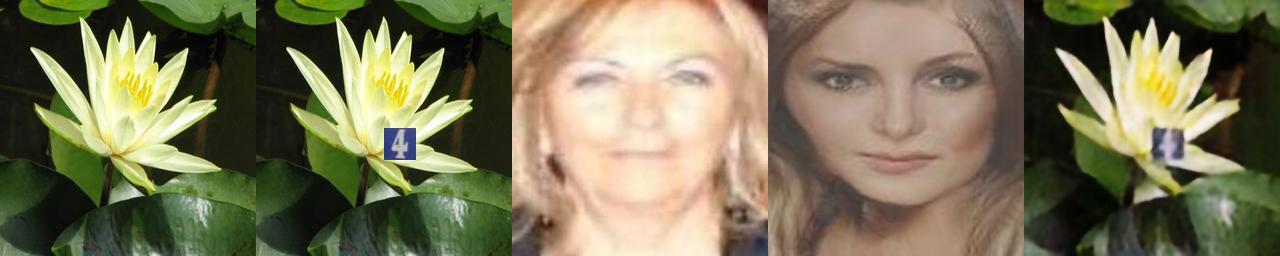
\includegraphics[scale=0.3]{figures/image_00284/BtoA_image_00284.jpg}
		\end{center}
		\caption{Images of test results generated by the method. The leftmost is base image. The second left is maskimage. The middle one is the reference image. The second one on the right is fake image generated by the B2A generator. The rightmost is the recovered image by the A2B generator.}
		\label{p1}
	\end{figure} 
	
		\begin{figure}
			\begin{center}
				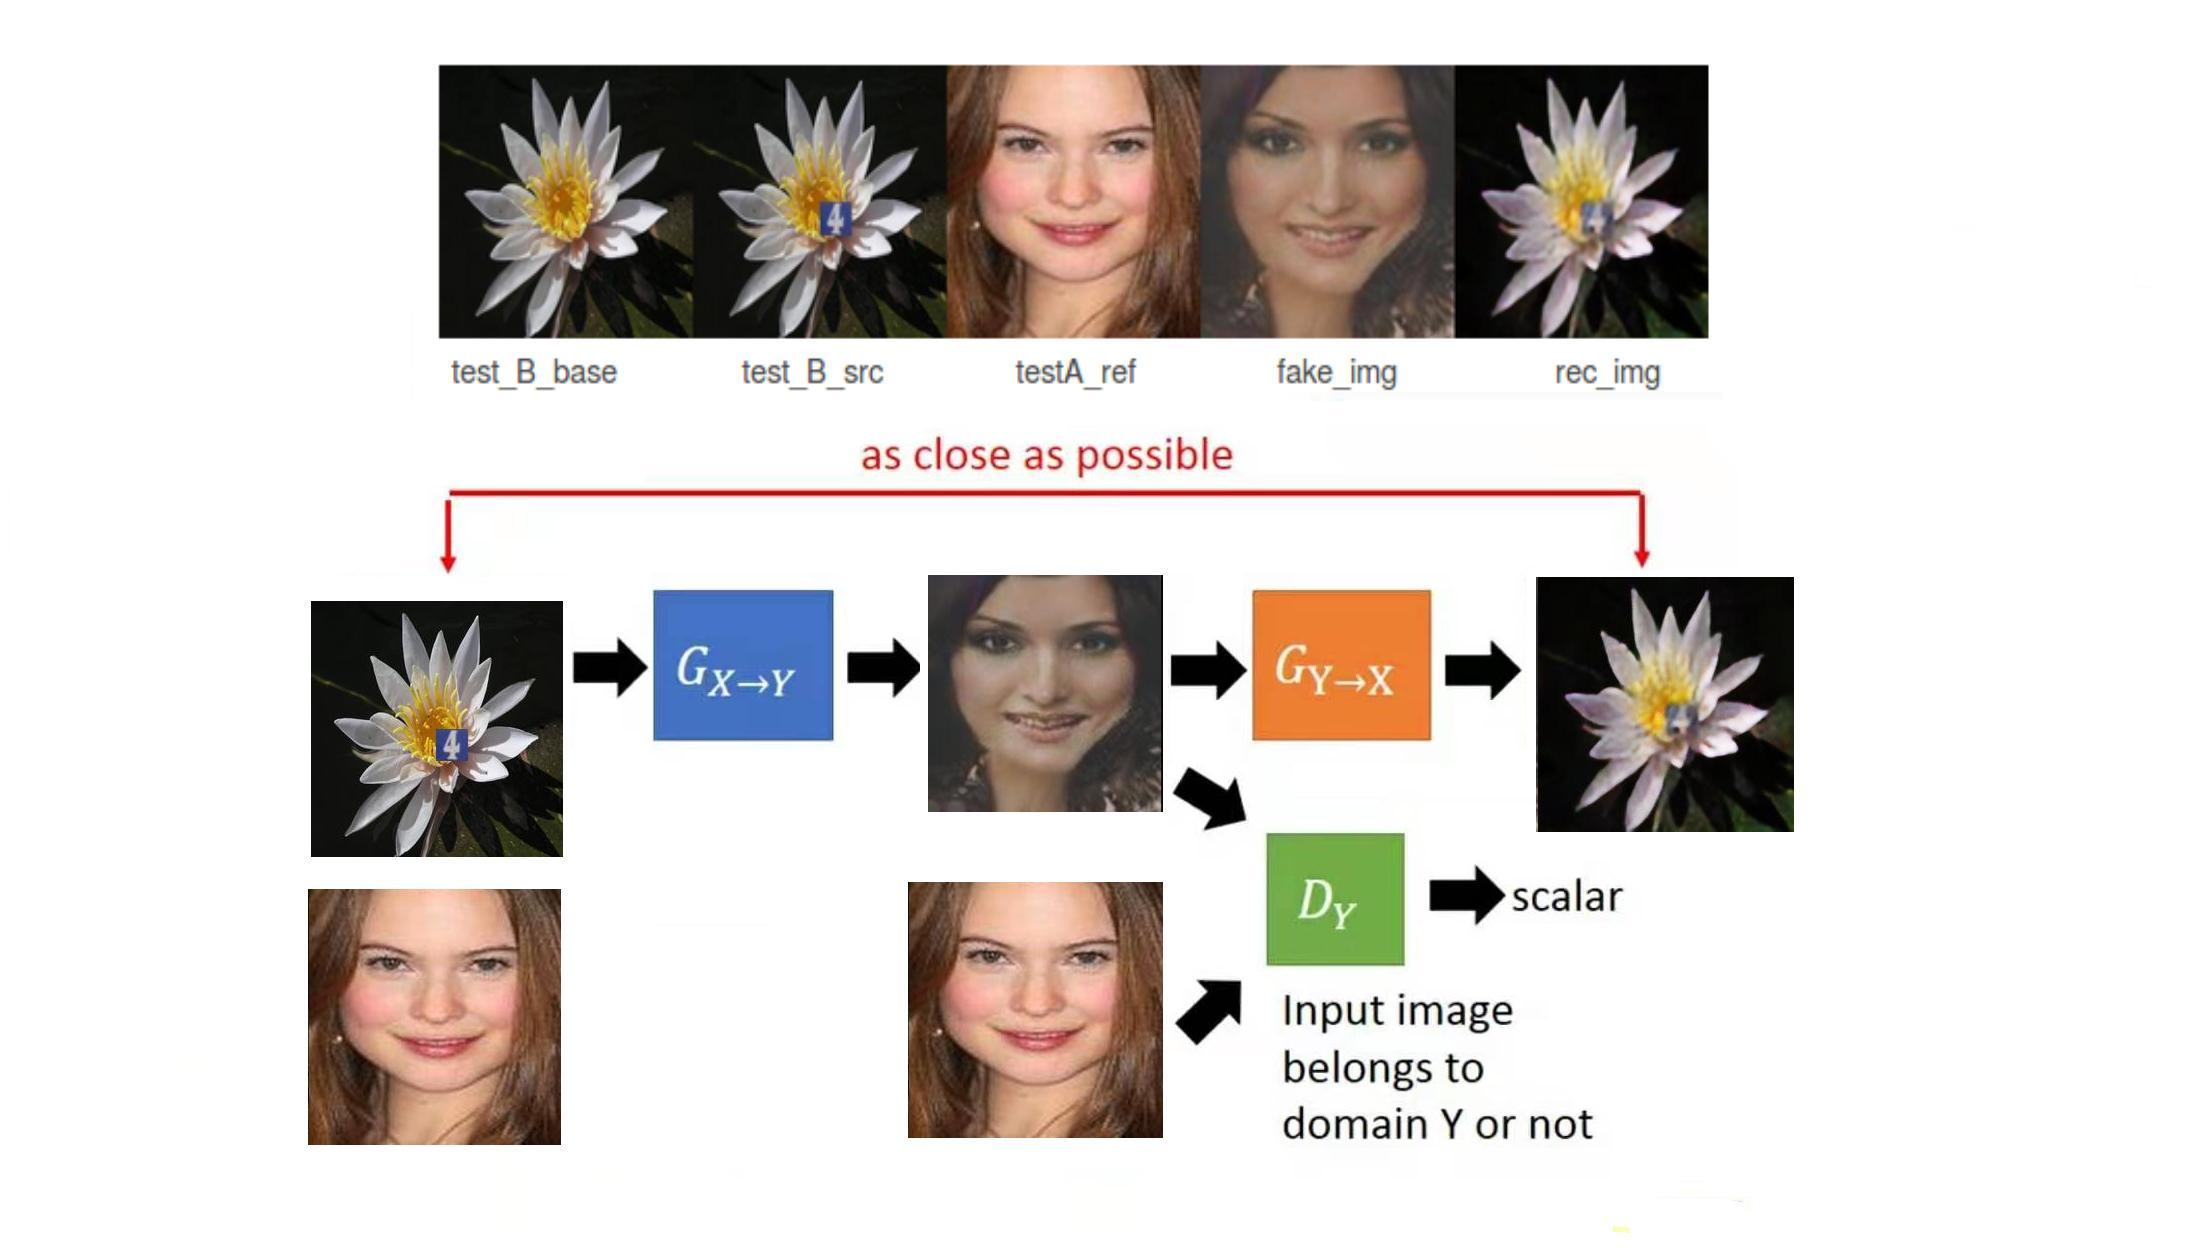
\includegraphics[scale=0.3]{figures/encripgan.jpg}
			\end{center}
			\caption{Overall implementation process of method.}
			\label{p9}
		\end{figure} 
	
	\begin{figure}
		\centering 
		\subfigure[]{ 
			\label{p2a} %% label for first subfigure 
			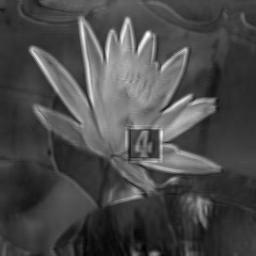
\includegraphics[width=5cm]{figures/image_00284/image_00284_c1_B2A_visual.jpg} 
		} 
		\subfigure[]{ 
			\label{p2b} %% label for second subfigure 
			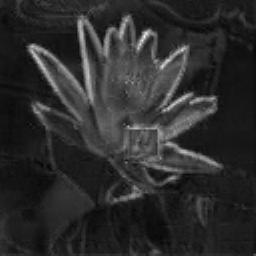
\includegraphics[width=5cm]{figures/image_00284/image_00284_c2_B2A_visual.jpg} 
		}
		\subfigure[]{ 
			\label{p2c} %% label for second subfigure 
			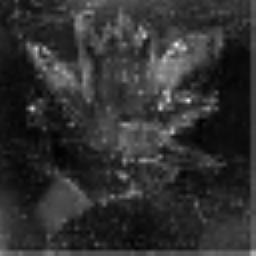
\includegraphics[width=5cm]{figures/image_00284/image_00284_c3_B2A_visual.jpg} 
		}
		\caption{Visual resutls of the former three layers of encoder in process of generating.}
		\label{p2}
	\end{figure}
	
	\begin{figure}
		\centering 
		\subfigure[]{ 
			\label{p3a} %% label for first subfigure 
			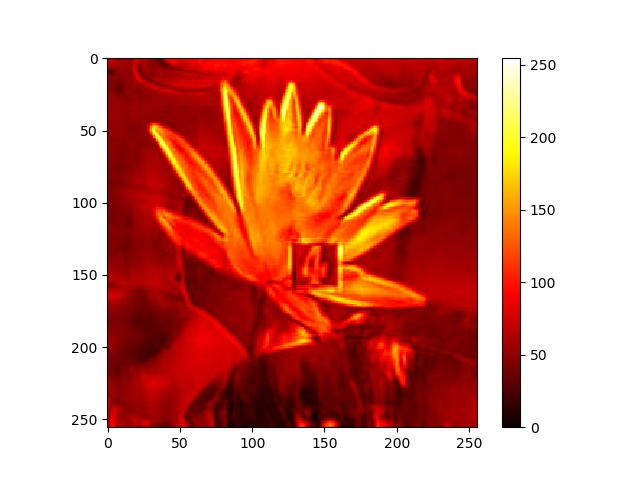
\includegraphics[width=5cm]{figures/image_00284/image_00284_c1_B2A_visual_heatmap.jpg} 
		} 
		\subfigure[]{ 
			\label{p3b} %% label for second subfigure 
			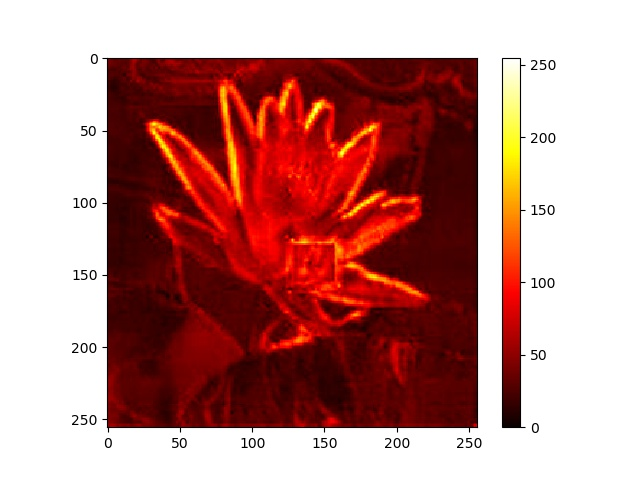
\includegraphics[width=5cm]{figures/image_00284/image_00284_c2_B2A_visual_heatmap.jpg} 
		}
		\subfigure[]{ 
			\label{p3c} %% label for second subfigure 
			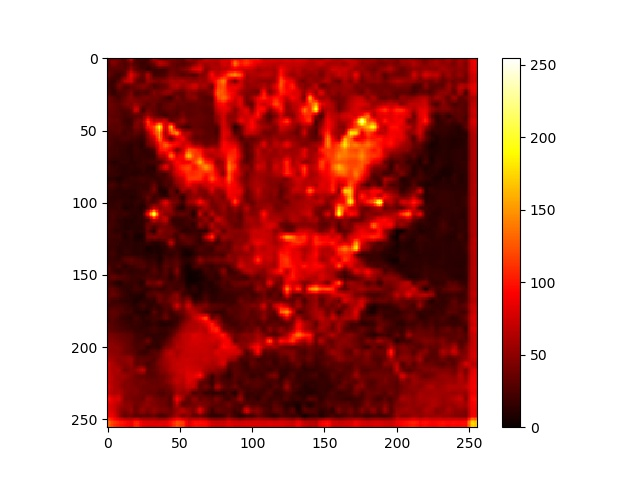
\includegraphics[width=5cm]{figures/image_00284/image_00284_c3_B2A_visual_heatmap.jpg} 
		}
		\caption{Visual heatmap resutls of the former three layers of encoder in process of generating.}
		\label{p3}
	\end{figure}
	
	Then it's natural for us to focus on the reconstruction process as shown in Fig.~\ref{p4}. The fake face image becomes as an input image or source image into the generator , which is generated in the process above, and the recover image is almost the same with the reference image.
	
	From Fig.~\ref{p4}\subref{p4a} to Fig.~\ref{p4}\subref{p4c}, the generator reconstructs or recovers the flower photograph with fake face image through the convolution network. We can see that CycleGAN may be able to reconstruct information from face, using feature map from Generator c1 to c3. The heatmap corresponding to the feature map as shown in Fig.~\ref{p5}. In a word, CycleGAN hide information which it needs to reconstruct in the generated image, fake face image in our experiment, in order to recover details in the reconstructed images.
	
	
	\begin{figure}
		\centering 
		\subfigure[]{ 
			\label{p4a} %% label for first subfigure 
			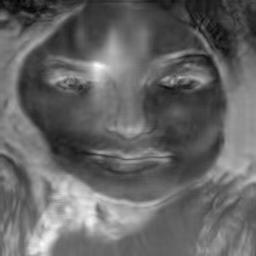
\includegraphics[width=5cm]{figures/image_00284/image_00284_c1_A2B_visual_recover.jpg} 
		} 
		\subfigure[]{ 
			\label{p4b} %% label for second subfigure 
			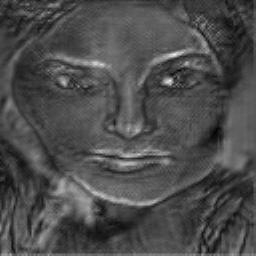
\includegraphics[width=5cm]{figures/image_00284/image_00284_c2_A2B_visual_recover.jpg} 
		}
		\subfigure[]{ 
			\label{p4c} %% label for second subfigure 
			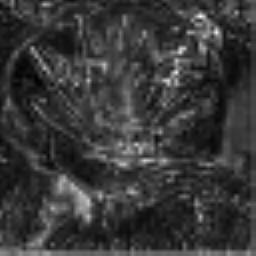
\includegraphics[width=5cm]{figures/image_00284/image_00284_c3_A2B_visual_recover.jpg} 
		}
		\caption{Visual resutls of the former three layers of encoder in process of recovering.}
		\label{p4}
	\end{figure}
	
	\begin{figure}
		\centering 
		\subfigure[]{ 
			\label{p5a} %% label for first subfigure 
			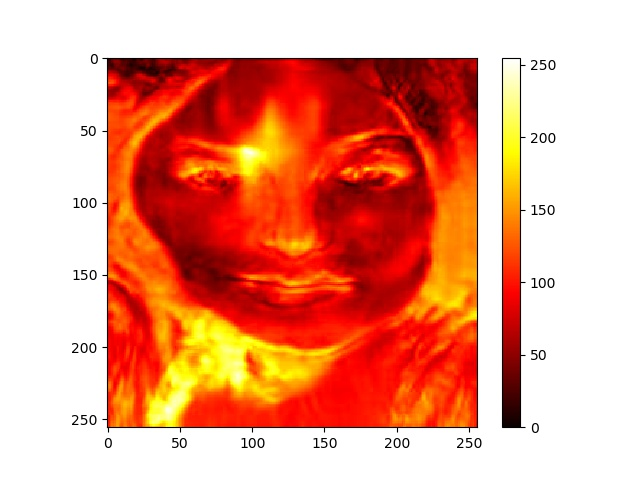
\includegraphics[width=5cm]{figures/image_00284/image_00284_c1_A2B_visual_recover_heatmap.jpg} 
		} 
		\subfigure[]{ 
			\label{p5b} %% label for second subfigure 
			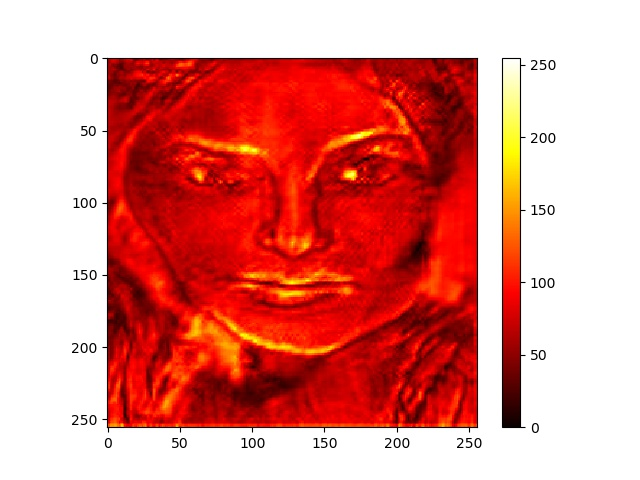
\includegraphics[width=5cm]{figures/image_00284/image_00284_c2_A2B_visual_recover_heatmap.jpg} 
		}
		\subfigure[]{ 
			\label{p5c} %% label for second subfigure 
			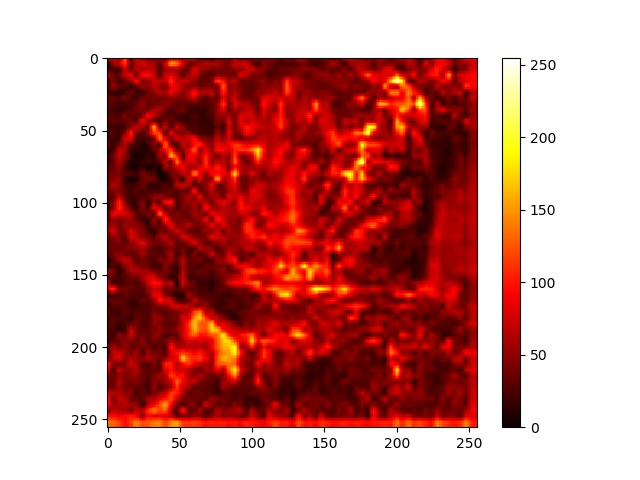
\includegraphics[width=5cm]{figures/image_00284/image_00284_c3_A2B_visual_recover_heatmap.jpg} 
		}
		\caption{Visual heatmap resutls of the former three layers of encoder in process of recovering.}
		\label{p5}
	\end{figure}
	
	\lstset{language=python}
	\begin{lstlisting}
	def save_seg_img_cla(base_src,vgg,name,direction):
	
	data2 = 0
	for item in ["e4", "e5", "e6"]:  
	data1 = vgg[0][item]
	data = data2 + data1             	
	data2 = data
	
	m, n = np.shape(data1)[1],np.shape(data1)[2]
	data_slice = np.reshape(data1, [m, n])
	data_norm = Normalize(data_slice)
	mul = np.ones((m,n))
	mul*=255.0
	data_norm=np.multiply(data_norm,mul)
	save_data = np.asarray(data_norm, np.int8)
	processed_r = Image.fromarray(save_data, "L")
	
	save_name_slice = name+"_"+item+"_"+direction + "_classif" 
	+ ".jpg"
	processed_r.save(save_name_slice)
	
	data_slice = mpimg.imread(save_name_slice)
	save_name_slice = name+"_"+item+"_"+direction+"_heatmap_" 
	+ "classif" + ".jpg"
	
	filename_txt = name+"_"+item+"_"+direction+"_heatmap_" 
	+ "classif" + ".txt"
	np.savetxt(filename_txt,data_slice)
	
	plt.imshow(data_slice, cmap=plt.cm.hot, vmin=0, vmax=255)
	plt.colorbar()
	#plt.imshow()
	
	plt.savefig(save_name_slice)
	#plt.show()
	plt.close()
	

	data_all = data
	m, n = np.shape(data_all)[1], np.shape(data_all)[2]
	data_all = np.reshape(data_all, [m, n])
	data_norm = Normalize(data_all)
	mul = np.ones((m, n))
	mul *= 255.0
	data_norm = np.multiply(data_norm, mul)
	
	save_data = np.asarray(data_norm, np.int8)
	processed_r = Image.fromarray(save_data, "L")
	
	save_name = name + "_" + direction + "_classif_all" + ".jpg"
	processed_r.save(save_name)
	
	data_all = mpimg.imread(save_name)
	save_name_1 = name + "_" + direction + "_heatmap_" 
	+ "classif_all" + ".jpg"
	
	filename_txt = name + "_" + direction + "_heatmap_" 
	+ "classif_all" + ".txt"
	np.savetxt(filename_txt, data_all)
	
	plt.imshow(data_all, cmap=plt.cm.hot, vmin=0, vmax=255)
	plt.colorbar()
	# plt.imshow()
	
	plt.savefig(save_name_1)
	# plt.show()
	plt.close()
	\end{lstlisting}\label{g1}
	

	\subsection{Analysis of Generator Sensitivity}
	
	In a steganographic task, it is important to correctly recover from encrypted image by relying on unique key pairs. Then we design an experiment to eval how sensitive the generator is to noise as shown in Fig.~\ref{p6}.
	
    We add different levels of gaussian white noise into the fake image which means the face image in orger to get a flower photograph with number. The fake face image in Fig.~\ref{p6}\subref{p6a} is added no noise, in the middle it has noise with std 0.01, and in the rightmost one it has noise with std 0.02. Comparing with these three images, we can realize that the generator is sensitive to noise only three levels when the image is quantized by 8-bit integers.
	
	However, the results wo got from this experiment is far from we want. The most crucial issue is that reference image does not work in the recover process just as Fig.~\ref{p6}\subref{p6c}, which should only recover from a red flower key but the yellow one also work during the recovering. This is the question we need to further study.
		
\begin{figure}
	\centering 
	\subfigure[]{ 
		\label{p6a} %% label for first subfigure 
		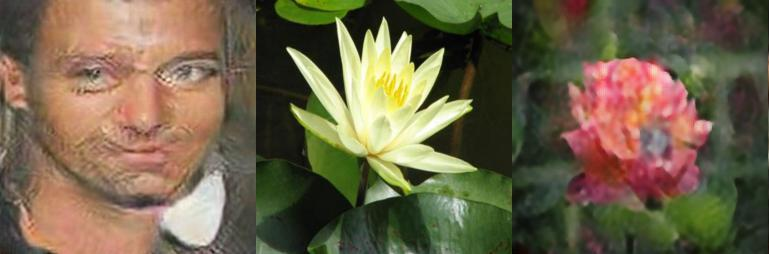
\includegraphics[width=5cm]{figures/20190330/image_01143_6_nonoise/save_3image.jpg} 
	} 
	\subfigure[]{ 
		\label{p6b} %% label for second subfigure 
		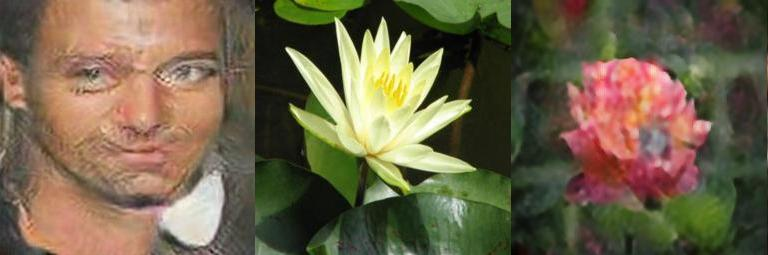
\includegraphics[width=5cm]{figures/20190330/image_01143_6_0.01noise/save_3image.jpg} 
	}
	\subfigure[]{ 
		\label{p6c} %% label for second subfigure 
		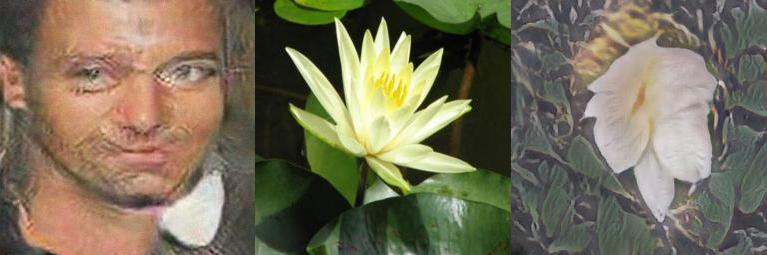
\includegraphics[width=5cm]{figures/20190330/image_01143_6_0.02noise/save_3image.jpg} 
	}
	\caption{The results of influences when add noises in the fake images. The leftmost with no noise. The middle image with noise(mean = 0, std= 0.01). And the rightmost image with noise(mean = 0, std= 0.02). And we can see the bad result in the rightmost image which has obscure recovered image.}
	\label{p6}
\end{figure}
	
	\lstset{language=python}
	\begin{lstlisting}
	sample_files_testB = glob('./datasets/{}/*.*'.format(
	self.dataset_dir + '/testB'))
	for flower_test in sample_files_testB:
	count += 1
	
	ref_image_2 = cv2.imread(flower_test)[:, :, ::-1]
	ref_image_2 = scipy.misc.imresize(ref_image_2, [256, 256])
	ref_image_2 = ref_image_2[np.newaxis, :, :, :]
	
	fake_img_2 = cv2.normalize(fake_img_2, None, 0, 255, 
	cv2.NORM_MINMAX, cv2.CV_8U)
	fake_img_2 = np.squeeze(fake_img_2)
	fake_img_noise = addGaussianNoise(fake_img_2, mean=0, 
	
	var=0.0004)
	fake_img_noise = fake_img_noise[np.newaxis, :, :, :]
	
	sample_image_an = np.concatenate([fake_img_noise, fake_img_noise, 
	ref_image_2], axis=2) 
	sample_image_an = sample_image_an/127.5 -1
	sample_image_an = np.array(sample_image_an).astype(np.float32)
	image_addnoise_path = args.test_dir+ "/" + name +"/" + 
	str(count) + "/"
	if not os.path.exists(image_addnoise_path):
	os.makedirs(image_addnoise_path)
	image_addnoise_savepath = os.path.join(image_addnoise_path,
	'{0}_{1}_{2}'.format(args.which_direction, 'sample_addnoise',
	os.path.basename(sample_file)))
	save_images(sample_image_an, [1, 1], image_addnoise_savepath)
	
	fake_img_B, rec_img_A, A2B_visual_A, B2A_visual_recover_B = 
	self.sess.run(
	[out_var_addnoise, rec_var_addnoise, self.A2B_visual, 
	
	self.B2A_recover_visual], feed_dict={self.test_A: sample_image_an})
	fake_img_addnoise = np.concatenate([sample_image_an, fake_img_B, 
	rec_img_A], axis=2)
	fake_img_addnoise_path = os.path.join(image_addnoise_path,  
	'{0}_{1}_{2}'.format(args.which_direction, 'addnoise_recover',
	os.path.basename(sample_file)))
	save_images(fake_img_addnoise, [1, 1], fake_img_addnoise_path)
	save_seg_img(A2B_visual_A, image_addnoise_path + name + str(count), 
	"A2B_addnoise_visual_") 
	save_seg_img(B2A_visual_recover_B, image_addnoise_path + name + 
	str(count), "B2A_addniose_visual_recover")  
	\end{lstlisting}\label{g2}
	
	\section{Plan}
	
	\begin{tabular}{rl}
		\textbf{Objective:} & Finish thesis for NeurIPS 2019.\\
		\textbf{Deadline:} & 2019.5.23
	\end{tabular}
	
	\begin{description}
		\item[\normalfont 2019.04.01---2019.04.07] Trying to analyze the influence of reference image and enhance its effects.
		\item[\normalfont 2018.04.08---2018.04.14] Finish quantitative analysis of encryption effect compared with NISP2017 paper.
		\item[\normalfont 2018.04.15---2018.04.21] Finish introduction and experimental part in paper.
		\item[\normalfont 2018.04.22---2018.04.28] Finish draft.
		\item[\normalfont 2018.04.29---2018.05.05] Finish adding quantitative index.
		\item[\normalfont 2018.05.06---2018.05.12] Finish model refinement and detailed figures and tables.
		\item[\normalfont 2018.05.13---2018.05.19] Finish checking references and grammar.
		\item[\normalfont 2018.05.20---2018.05.23] Finish final draft for NeurIPS 2019 paper.
	\end{description}
	
	% If you don't cite any references, please comment the following two lines
	\bibliographystyle{ieee}
	\bibliography{ref.bib}
	
\end{document}